\section{Degenerate Fermi Gas}
% Start working on HW2! Due Oct. 3
\subsection{Review of the Weakly Interacting Fermion Construction}
Last time, we started looking at the Fermi gas; it is what you get when you throw away the interactions between fermions (if you retain the interactions, you have something known as a Fermi liquid). Recall that we quantized the field:
\begin{equation}
    \psi_\sigma(\v{x}, t) = \int \frac{d^3k}{(2\pi)^{3/2}}e^{i\v{k} \cdot \v{x} - i\frac{\hbar\v{k}^2}{2m}t} \alpha_\sigma(\v{k}).
\end{equation}
We recall that we showed how no two fermions could occupy the same state. So building up the ground state of an $N$-particle fermion state, we start with the lowest energy state and place one (actually two, accounting for spin) particle per energy level. Since $\e \propto \v{k}^2$, all states up to a spherical surface known as the \emph{Fermi sphere} become filled. 

We tried to construct this state (the vacuum), but it resulted in some mathematical ugliness (with an infinite continuous product of creation operators up to some $\v{k}$... mathematical nonsense). But we got around this by talking about the state directly and postulating its properties. We say that:
\begin{equation}
    \begin{split}
        &\alpha_\sigma^{\dag}(\v{k})\ket{\O} = 0 \quad \abs{\v{k}} \leq k_F
        \\ &\alpha_\sigma(\v{k})\ket{\O} = 0 \quad \abs{\v{k}} > k_F.
    \end{split}
\end{equation}
though whether the states on the Fermi sphere are filled or empty will not be of particular importance to us. 

\subsection{Particles and Holes}
Let us now rename some things:
\begin{equation}
    \begin{split}
        &\alpha_\sigma(\v{k}) = a_\sigma(\v{k}) \quad \text{if $\abs{\v{k}} > k_F$}
        \\ &\alpha_\sigma(\v{k}) = b_\sigma^\dag(-\v{k}) \quad \text{if $\abs{\v{k}} < k_F$}
    \end{split}
\end{equation}
so it looks like we have two kinds of creation/annhilation operators. They are in a sense the same, but we label them like this to make the defining formulas for $\ket{\O}$ simpler, as now we can write them as:
\begin{equation}
    \begin{split}
        &a_\sigma(\v{k})\ket{\O} = 0 \quad \abs{\v{k}} > k_F
        \\ &b^{\dag}_\sigma(\v{k})\ket{\O} = 0 \quad \abs{\v{k}} < k_F.
    \end{split}
\end{equation}
And we can write an excited state as:
\begin{equation}
    (a^{\dag\sigma_1}(\v{k}_1)\ldots b^{\dag}_{\rho_1}(\v{l}_1))\ket{\O}
\end{equation}
where the $a$s create fermions, and the $b$s create holes (annihilating what was already there). We can therefore write the quantized field operator as:
\begin{equation}
    \psi_\sigma(\v{x}, t) = \int_{\abs{\v{k}} > k_F} \frac{d^3k}{(2\pi)^{3/2}}e^{i\v{k} \cdot \v{x} - i\frac{\hbar\v{k}^2}{2m}t} a_\sigma(\v{k}) + \int_{\abs{\v{k}} < k_F} \frac{d^3k}{(2\pi)^{3/2}}e^{-i\v{k} \cdot \v{x} - i\frac{\hbar\v{k}^2}{2m}t} b^{\dag}_\sigma(\v{k})
\end{equation}
where we have done a change of variables $\v{k} \to -\v{k}$ in the second integral. So, $\psi$ has two parts; it either annhilates a particle, or creates a hole. The only funny part of the expression is that the phases have opposite signs, but the energy part does not. It looks like the holes somehow gives us back negative energy. There is something we can do to repair this; let us redefine the energy. As it is currently, we have $\e = \frac{\hbar^2\v{k}^2}{2m}$. What if instead we add a constant\footnote{Which we are told all the time in QM we are allowed to do; note that really this is a lie, but let us not worry about it.}:
\begin{equation}
    \frac{\hbar^2\v{k}^2}{2m} \to \frac{\hbar^2\v{k}^2}{2m} - \frac{\hbar^2k_F^2}{2m} = \frac{\hbar^2\v{k}^2}{2m} - \e_F
\end{equation}
if we do this and plug this into the energy, we get something nicer, as both particles and holes will have positive energy relative to the vacuum state (we return to this statement shortly). The net effect on the Hamiltonian is the substitution:
\begin{equation}
    H \to H - \e_F\mathcal{N}.
\end{equation}
Now, if we want to calculate the number operator, we have:
\begin{equation}
    \mathcal{N} = \int_{\abs{\v{k}} > k_F} d^3k a^{\dag\sigma}(\v{k})a_\sigma(\v{k}) - \int_{\abs{\v{k}} < k_F} d^3k b^\dag_\sigma(\v{k})b^\sigma(\v{k}) + \rho V
\end{equation}
The negative sign on the $b$ integral comes from the fact that we interchange the order to get the correct order of operators, but then we get a negative sign from the anticommutation, and we add $\rho V$ (with $\rho$ the density and $V$ the volume... an infinite constant. It is counting all of the particles in the Fermi sea/inside the Fermi sphere). If we now write down the Hamiltonian, we have:
\begin{equation}
    H - \e_F \mathcal{N} =  \int_{\abs{\v{k}} > k_F} d^3k \frac{\hbar^2(\v{k}^2 - k_F^2)}{2m}a^{\dag\sigma}(\v{k})a_\sigma(\v{k}) - \int_{\abs{\v{k}} < k_F} \frac{\hbar^2(k_F^2 - \v{k}^2)}{2m}b_\sigma^\dag(\v{k})b^\sigma(\v{k}) + \varphi V
\end{equation}
where the change in the sign of the energy is from the anticommutation of the $b$s, and we also add the energy (an infinite constant representing the energy of all particles within the Fermi sphere) to compensate for this anticommutation. Where:
\begin{equation}
    \Phi = \avg{H - \e_F N} = \varphi V
\end{equation}
is the Grand canonical free energy. Note if we open our system, the fermions were go out of the system until none are left (they tend to want to escape to minimize the free energy); in order for this to not happen, there is a chemical potential $\mu$ which can be seen as a sort of ``gate voltage'' of the fermions. It is an adjustable parameter we can tweak to coax the fermions back in. So then, determining the density has to do with extremizing the free energy.

Having do this, we notice that the energy of our excitations are all positive! So our shifting of the Hamiltonian was a good choice.

\subsection{Equations of State and Physical Parameters}
How do we figure out the parameters in the above expression (e.g. the density)? Let's return to the particle number in our old formalism:
\begin{equation}
    \mathcal{N} = \int d^3k \alpha^{\dag\sigma}(\v{k})\alpha_\sigma(\v{k})
\end{equation}
From this, let's calculate the expectation value for the vacuum state\footnote{Note we will be very mathematically relaxed in our manipulations here... e.g. interchanging orders of matrix elements. It may be possible to justify this with working in a finite system and then taking limits, but we get the same answer so let us be cavalier about it.}:
\begin{equation}
    \rho V = \bra{\O}\mathcal{N}\ket{\O} = \int_{\abs{\v{k}} < k_F}(2J + 1)\delta^3(\v{0})
\end{equation}
where we have noted that the integral vanishes when $\abs{\v{k}} > k_F$ due to how the vacuum is defined, and we have replaced the $\alpha$s with a terrible anticommutator. Here $\delta^3(\v{k})$ is defined as:
\begin{equation}
    \delta^3(\v{k}) = \int \frac{d^3x}{(2\pi)^3}e^{i\v{k} \cdot \v{x}}
\end{equation}
so then:
\begin{equation}
    \delta^3(\v{0}) = \int \frac{d^3x}{(2\pi)^3} = \frac{V}{(2\pi)^3} 
\end{equation}
so the above expectation value becomes:
\begin{equation}
    \rho V = \int_{\abs{\v{k}} < k_F}(2J + 1)\frac{V}{(2\pi)^3} 
\end{equation}
and if we now cancel out the volume, we remove the infinite quantities from both sides:
\begin{equation}\label{eq-rho}
    \rho = \int_{\abs{\v{k}} < k_F}\frac{2J + 1}{(2\pi)^3} = \frac{(2J+1)}{(2\pi)^3} \frac{4\pi}{3}k_F^3 = \frac{(2J+1)}{6\pi^2}k_F^3
\end{equation}
where $\frac{4\pi}{3}k_F^3$ is the volume contained in the Fermi-sphere of radius $k_F$. Another calculation we can do is to calculate the internal energy; this is just the expectation value of our original Hamiltonian, which works out in a very similar way:
\begin{equation}
    U = \bra{\O}H\ket{\O} = V\frac{(2J+1)}{(2\pi)^3}\int_{\abs{\v{k}} < k_F}d^3k \frac{\hbar^2 \v{k}^2}{2m}.
\end{equation}
We go to polar coordinates to calculate the above:
\begin{equation}
    U = V\frac{(2J+1)}{(2\pi)^3} \frac{\hbar^2}{2m}\int_0^{k_F} k^2 dk \int_0^\pi \sin(\theta)d\theta \int_0^{2\pi} d\phi k^2 = V\frac{(2J+1)}{(2\pi)^3} \frac{\hbar^2}{2m}\left(\frac{k_F^5}{5}\right)\left(4\pi\right)
\end{equation}
So we conclude:
\begin{equation}\label{eq-uV}
    U = V\frac{(2J+1)}{(2\pi)^2}\frac{\hbar^2}{m}\frac{k_F^5}{5} = uV
\end{equation}
where $u$ is the energy density. So, we can now use these two results to solve for $k_F$ and then eliminate it from our expressions. This gives us equations of state, which contain valuable (nontrivial!) physical information. We find from Eq. \eqref{eq-rho}:
\begin{equation}\label{eq-kF}
    k_F = \left[\frac{6\pi^2\rho}{(2J+1)}\right]^{1/3}
\end{equation}
and so plugging into Eq. \eqref{eq-uV} we have:
\begin{equation}\label{eq-u}
    u = \frac{\hbar^2}{2m}\frac{(2J+1)}{10\pi^2}\left[\frac{6\pi^2\rho}{(2J+1)}\right]^{5/3}
\end{equation}
so $u \propto \rho^{5/3}$. We can then find various other physical quantities by using thermodynamic relations, e.g. the pressure as a function of energy density (note we have assumed that everything is at constant zero temperature here):
\begin{equation}\label{eq-P}
    P = \left.-\dpd{U}{V}\right|_N = \frac{2}{3}u
\end{equation}
We can also find the chemical potential:
\begin{equation}\label{eq-muef}
    \mu = \left.\dpd{U}{N}\right|_V = \e_F
\end{equation}
where in the above calculation we would write $U = uV$, and then write $\rho = N/V$. So we find at zero temperature that indeed the chemical potential is the Fermi energy (of course if one turns on interactions, or the temperature, then this will no longer hold!) What's more, if we look at $\Phi$, we have:
\begin{equation}\label{eq-phi}
    \Phi = \avg{H - \mu \mathcal{N}} = \varphi V \implies \varphi = -P
\end{equation}

\subsection{A Simple Example of a Quantum Phase Transition}
Note that there is a more detailed discussion of the above in the notes, and we have covered the main points here. But let us discuss one thing that is not in the notes. We recall the interplay between the fermions wanting to get away and the chemical potential to coax them back in. We now consider a simple model of a \emph{quantum phase transition}\footnote{One of the main models discussed in Sachdev's book by this title!}. We assume that we can tune the chemical potential; as we tune, the density varies. If $\mu = 0$, the density is zero. If we make it negative, the density stays at zero. So, as we increase $\mu$, the density becomes nonzero as we cross $\mu = 0$; signalling a phase transition in the system.

\begin{figure}[htbp]
    \centering
    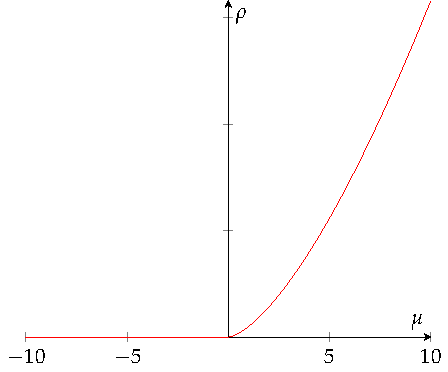
\includegraphics[]{Images/fig-rhomu.pdf}
    
    \caption{Plot of $\rho$ vs. $\mu$ (arbitrary units). $\rho$ is zero for $\mu \leq 0$ and $\rho \propto \mu^{3/2}$ for $\mu > 0$, signalling a phase transition in the system.}
    \label{fig-rhomu}
\end{figure}

The fact that $\rho \propto \mu^{3/2}$ is obtainable by realizing that $k_F \propto \rho^{1/3}$ (Eq. \eqref{eq-kF}) and $\mu = \e_F \propto k_F^2$ (Eqs. \eqref{eq-muef} and the definition of Fermi energy). Since $\phi \propto P \propto u$ (Eqs. \eqref{eq-phi} and \eqref{eq-P}), and $u \propto \rho^{5/3}$ (Eq. \eqref{eq-rho}), we find that the free energy $\phi$ is related to the chemical potential by $\phi \propto \mu^{5/2}$.

Since we have to take three derivatives of $\phi$ w.r.t. $\mu$ before we get a discontinuity (at $\mu = 0$), by the Ehrenfest classification of phase transitions, this is a third order phase transition. This discussion can also be taken as something that highlights the difference between Fermi gas and Fermi liquid behaviour; interactions change the properties of the system significantly.